\section{Results}
\label{sec-results}
%\input graphsize_table

We will analyse search performance as follows: 
First, we look at the effectiveness of our new online and offline symmetry
reduction methods using results published in \cite{harabor10} as a 
comparative baseline.
Next, we compare and contrast the performance of our new algorithm with that
of another similar method recently described in the literature \cite{pochter10}.
Finally, we demonstrate the relative strengths and weaknesses of these two
techniques by scaling all maps in our benchmark sets by a factor of 3 and looking
at the effect this has on performance.


\begin{figure*}[t]
       \begin{center}
                       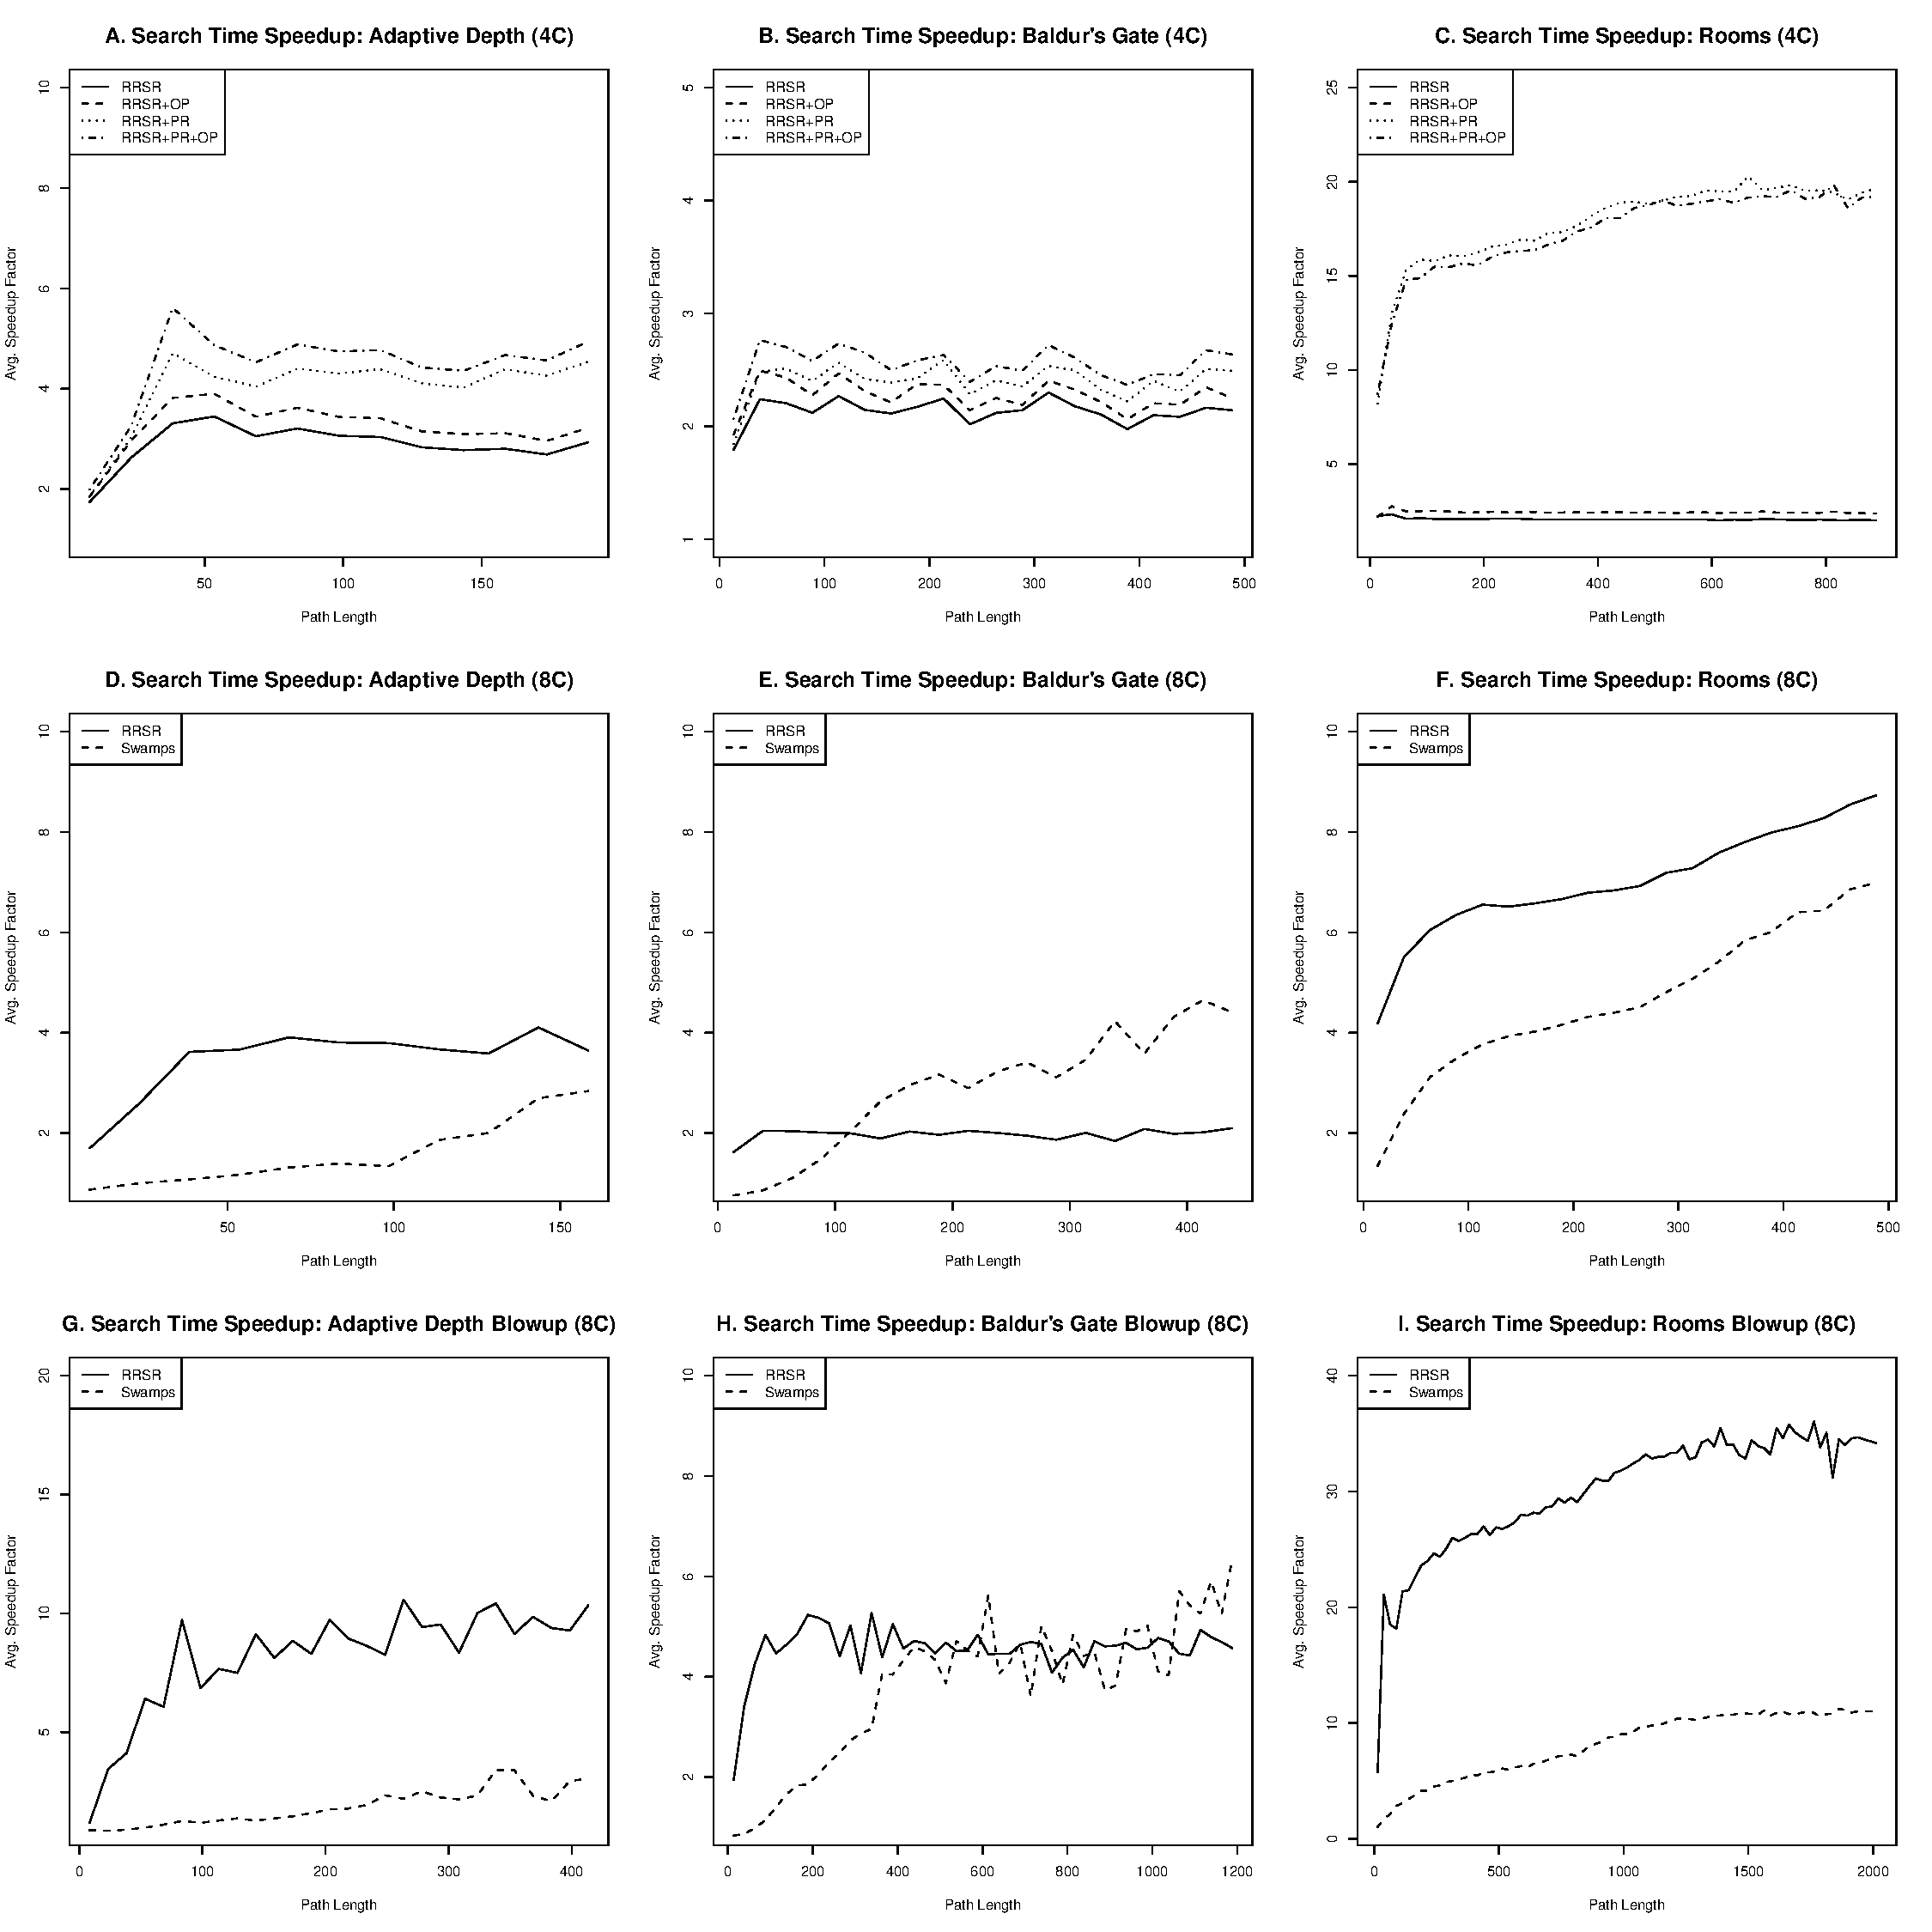
\includegraphics[width=1.95\columnwidth, trim = 10mm 10mm 10mm 0mm]{diagrams/speedup.pdf}
       \end{center}
       \caption{Average A* speedup on each of our three benchmarks. 
		Results are given in terms of nodes expanded and search time.}
\label{fig-speedup}
\end{figure*}

\textbf{Symmetry Reduction Improvements: }
In Figure \ref{fig-speedup} (A to C) we report on the  
effectiveness of offline perimeter reduction (PR) and on-the-fly 
node pruning (OP) to speeding up A* search on 4-connected grid maps.
Our baseline comparison is the Rectangular Room Symmetry Reduction algorithm 
(RRSR) originally described in \cite{harabor10}.
Some clear trends immediately emerge: first, the single biggest improvement in each
case is observed when applying perimeter reduction to the basic RRSR method.
In the case of the Rooms benchmark (Figure \ref{fig-speedup}C) RRSR+PR is over 9
times faster than RRSR alone and up to 19 times faster than A* search on an unmodified
grid map.
Smaller but still significant gains are also observed on the remaining two benchmarks:
on Adaptive Depth (Figure \ref{fig-speedup}A) RRSR+PR is twice as fast as RRSR alone
and performance on Baldur's Gate (Figure \ref{fig-speedup}B) is improved by over 10\%.
By comparison, on-the-fly node pruning yields much smaller gains across the same benchmarks:
both RRSR+OP and RRSR+PR+OP only improve the search performance by 10\% on the majority
of problem instances.
Finally, it is interesting to note the sometimes large performance variation 
from one benchmark to another. This is indicative of how effectively we can 
decompose the different maps into rectangular shaped regions.
For example, the maps in the Rooms set are highly suited to this approach but those
from Baldur's Gate, which have an unusual 45-degree orientation, are not.

